\documentclass{ctexart}
\usepackage{amsmath}
\usepackage{amssymb}
\usepackage{pgfplots}
\usepackage[margin=1in]{geometry}
\usepackage{physics}
\usepackage{titlesec}

\pgfplotsset{compat=newest}
\usepgfplotslibrary{polar}
\titleformat{\section}[runin]{\large\bfseries}{\zhnumber{\thesection}}{1em}{}

\title{23-24 秋冬数分期末参考答案}
\author{silvermilight}
\date{2024 年 1 月 27 日}

\begin{document}

\maketitle

答案仅供参考,不保证完全正确,也不一定是最优解,欢迎指出错误或提出更好的解法. ---rzm

\section{(10 points)}
    叙述数列收敛的柯西收敛准则;并用该准则证明:数列$\displaystyle\left\{\sum_{k=1}^n \frac{(-1)^{k+1}}{k^{2024}}\right\}$收敛.
\paragraph{Solution}
    Cauchy 收敛准则:若$\forall\varepsilon>0,\exists N>0,\forall n>N,m>N $ 都有 $|a_n-a_m|<\varepsilon$,则数列$\{a_n\}$收敛.

    设数列 $a_n=\displaystyle\sum_{k=1}^n \dfrac{(-1)^{k+1}}{k^{2024}}$ ,不妨设 $m<n$ ,则
    \begin{align*}
        |a_n-a_m| &= \left| \sum_{k=m+1}^n \frac{(-1)^{k+1}}{k^{2024}} \right| \\
                    & \leqslant \sum_{k=m+1}^n \frac{1}{k^{2024}} < \sum_{k=m+1}^n \frac{1}{k^2} \\
                    & < \sum_{k=m+1}^n \left( \frac{1}{k-1}-\frac{1}{k} \right) \\
                    & = \frac{1}{m}-\frac{1}{n} < \frac{1}{m}
    \end{align*}

    因此,只需令 $\dfrac{1}{m}<\varepsilon$,故取 $N=\left\lfloor \dfrac{1}{\varepsilon} \right\rfloor$,则 $\forall n>N,m>N$都有$|a_n-a_m|<\varepsilon$,据 Cauchy 收敛定理知原命题成立.

\section{(35 points)}
    \begin{enumerate}
        \item 求极限 $\displaystyle\lim_{n \to +\infty} n\sum_{k=1}^n \dfrac{1}{n^2+k^2}$.
        \paragraph{Solution}
        设 $f(x)=\dfrac{1}{1+x^2}$ ,则 $f(x) \in C[0,1]$ ,故 $f(x)$ 可积且有原函数 $\arctan{x}$.

        由于 $\dfrac{n}{n^2+k^2}=\dfrac{1}{n}\cdot \dfrac{1}{1+\left( \frac{k}{n} \right)^2}
                                =f\left(\frac{k}{n}\right)$,故

        \[
            \text{原式} = \int_{0}^{1} f(x) \dd{x} = \eval{\arctan{x}}_0^1 = \dfrac{\pi}{4}
        \]

        \item 求极限 $\displaystyle\lim_{x \to 1} \dfrac{x^x-x}{1-x+\ln{x}}$.
        \paragraph{Solution}
        令 $t=x-1$ ,则 $t \to 0$ ,用两次 L'Hospital 法则

        \begin{align*}
            \text{原式} &= \lim_{t \to 0} \frac{(t+1)^{t+1}-t-1}{-t+\ln(1+t)} \\
                        &= \lim_{t \to 0} \frac{(1+\ln (t+1))(t+1)^{t+1}-1}{-1+\frac{1}{t+1}} \\
                        &= \lim_{t \to 0} \frac{((1+\ln (t+1))^2+\frac{1}{t+1})(t+1)^{t+1}}{-\frac{1}{(t+1)^2}} \\
                        &= -2
        \end{align*}

        \item 求极限 $\displaystyle\lim_{x \to 0} \dfrac{\displaystyle\int_0^{x^2} t^2 e^{\sin t} \dd{x}}{\ln (1+x^6)} $.
        \paragraph{Solution}
        设 $f(x)=\displaystyle\int_0^{x^2} t^2 e^{\sin t} \dd{x}$ ,由于被积函数在 $\mathbb{R}$ 上连续,知 $f(x) \in D( \mathbb{R} )$ ,且 $f'(x)=2x^5 e^{\sin x^2}$

        当 $x \to 0$ 时,分子和分母都趋向0,可以使用 L'Hospital 法则

        \[
            \text{原式} = \lim_{x \to 0} \frac{2x^5 e^{\sin x^2}}{\frac{6x^5}{1+x^6}}
                        = \lim_{x \to 0} \frac{(1+x^6) e^{\sin x^2}}{3}
                        = \frac{1}{3}
        \]

        \item 求 $\displaystyle\int_1^{+\infty} \dfrac{\arctan x}{x^2} \dd{x}$.
        \paragraph{Solution}
        \begin{align*}
            \text{原式} &= - \int_1^{+\infty} \arctan x \dd(\frac{1}{x}) \\
                        &= - \eval{\left( \frac{\arctan x}{x} \right)}_1^{+\infty} + \int_1^{+\infty} \frac{1}{x(1+x^2)} \dd{x} \\
                        &= \frac{\pi}{4} + \frac{1}{2} \int_1^{+\infty} \frac{1}{x^2 (1+x^2)} \dd{x}^2 \\
                        &= \frac{\pi}{4} + \frac{1}{2} \int_1^{+\infty} \left(\frac{1}{x^2}-\frac{1}{1+x^2} \right) \dd{x}^2 \\
                        &= \frac{\pi}{4} + \frac{1}{2} \eval{\left(\ln \frac{x^2}{1+x^2} \right)}_1^{+\infty} \\
                        &= \frac{\pi}{4} + \frac{1}{2} \ln 2
        \end{align*}

        \item 求双纽线 $r=\sqrt{\cos (2\theta)}$ 所围平面图形的面积.
        \paragraph{Solution}
        \begin{figure}[htbp]
            \centering
            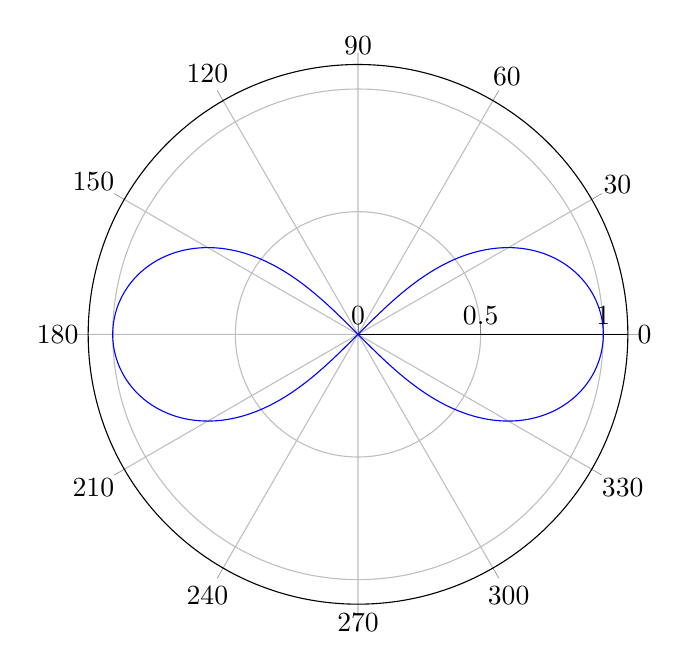
\begin{tikzpicture}
                \begin{polaraxis}
                \addplot+[mark=none,color=blue,domain=-45:45,samples=1000]{sqrt(cos(2*x))};
                \addplot+[mark=none,color=blue,domain=135:225,samples=1000]{sqrt(cos(2*x))};
                \end{polaraxis}
            \end{tikzpicture}
            \caption{双纽线}
            \label{fig:function1}
        \end{figure}
        图 \ref{fig:function1} 表明双纽线关于$x$轴与$y$轴对称,故我们可以只计算位于第一象限的部分面积.

        \[
            \text{原式} = 4 \int_{0}^{\frac{\pi}{4}} \frac{1}{2} \cos(2\theta) \dd{\theta}
                        = \eval{\sin(2\theta)}_0^{\frac{\pi}{4}}
                        = 1
        \]

    \end{enumerate}


\section{(10 points)}
    证明 Cantor 定理:若 $f(x)$ 在 $[0,1]$ 上连续,则 $f(x)$ 在 $[0,1]$ 上一致连续.
\paragraph{Solution}

设 $E = \{ t\in (a,b] \mid f(x) \text{~在~}[a,t]\text{~上一致连续} \} $.

由 $f(x)\in C[0,1]$ ,据 Cauchy 收敛定理知 $\forall \varepsilon>0, \exists \delta>0, \forall x_1,x_2 \in [0,\delta), |f(x_1)-f(x_2)|<\varepsilon$,
故 $f(x)$ 在 $[0,\delta)$ 上一致连续,所以 $\frac{\delta}{2} \in E$.

$E\neq\varnothing$ 且有上界 1,由确界原理知 $E$ 有上确界,记 $\sup{E}=\alpha$.

下证 $\alpha=1$.

假设 $\alpha \in (0,1)$,则 $\forall \varepsilon>0$,

由 $f(x)\in C[0,1]$ ,据 Cauchy 收敛定理,取 $\varepsilon_0=\varepsilon$,则 $\exists \delta_0>0, \forall x_1,x_2 \in (\alpha-\delta_0,\alpha+\delta_0), |f(x_1)-f(x_2)|<\varepsilon_0$.

由 $\alpha$ 为 $E$ 的上确界,$\exists \beta>\alpha-\frac{\delta}{2}, \beta\in E$ ,即 $f(x)$ 在 $[0,\beta]$ 上一致连续.
取 $\varepsilon_1=\varepsilon$,则 $\exists \delta_1>0, \forall x_1,x_2 \in [0,\beta]$且$|x_1-x_2|<\delta_1, |f(x_1)-f(x_2)|<\varepsilon_1$

取 $\delta=\min\{\frac{\delta_0}{2},\delta_1\}$,则 $\forall x_1,x_2 \in [0,\beta]$且$|x_1-x_2|<\delta$,$x_1$ 与 $x_2$ 必定同时落在 $[0,\beta]$ 内或 $(\alpha-\delta_0,\alpha+\delta_0)$ 内.
故 $|f(x_1)-f(x_2)|<\varepsilon$. 因此 $f(x)$ 在 $[0,\alpha+\frac{\delta_0}{2}]$ 上一致连续.

由此可知 $\alpha+\frac{\delta_0}{2} \in E$,与 $\alpha=\sup E$ 矛盾. 故 $\alpha=1$,$f(x)$ 在 $[0,1]$ 上一致连续.

\section{(10 points)}
    求函数 $f(x)=\displaystyle\int_{-1}^1 |x-t|e^{t^2} \dd{t}$ 在 $\mathbb{R}$ 上的最小值.
\paragraph{Solution}
    分以下三种情况讨论:
    \begin{enumerate}
        \item $x \geqslant 1$,则
        \[
            f(x) = x\int_{-1}^1 e^{t^2} \dd{t} - \int_{-1}^1 te^{t^2} \dd{t}
                            = x\int_{-1}^1 e^{t^2} \dd{t} - \frac{1}{2} \eval{e^{t^2}}_{-1}^1
                            \geqslant \int_{-1}^1 e^{t^2} \dd{t}
        \]
        \item $x \leqslant -1$,则
        \[
            f(x) = \int_{-1}^1 te^{t^2} \dd{t} - x\int_{-1}^1 e^{t^2} \dd{t}
                            = \frac{1}{2} \eval{e^{t^2}}_{-1}^1 - x\int_{-1}^1 e^{t^2} \dd{t}
                            \geqslant \int_{-1}^1 e^{t^2} \dd{t}
        \]
        \item $-1<x<1$,则
        \begin{align*}
            f(x) &= x\int_{-1}^x e^{t^2} \dd{t} - \int_{-1}^x te^{t^2} \dd{t} + \int_x^1 te^{t^2} \dd{t} - x\int_x^1 e^{t^2} \dd{t} \\
                    &= x \left(\int_{-1}^x e^{t^2}\dd{t} - \int_x^1 e^{t^2}\dd{t} \right) + e - e^{x^2}
        \end{align*}

        求导可得 $f'(x) = \displaystyle\int_{-1}^x e^{t^2}\dd{t} - \int_x^1 e^{t^2}\dd{t},\quad f''(x)=2e^{x^2}>0$,故 $f'(x)$ 单调递增.

        由 $f''(x)=2e^{x^2}$ 为偶函数,知 $f'(0)=0$,故 $f(x)$ 在 $[-1,0]$ 上单调递减,在 $[0,1]$ 上单调递增,在 $x=0$ 处取得最小值 $e-1$.
    \end{enumerate}

    由于 $\displaystyle\int_{-1}^1 e^{t^2} \dd{t} = 2\int_0^1 e^{t^2} \dd{t} > 2\int_0^1 te^{t^2} \dd{t} = e-1$,故 $e-1$ 为 $f(x)$ 在 $\mathbb{R}$ 上的最小值.

\section{(10 points)}
    证明导函数极限定理:若函数 $f(x)$ 在 $\mathbb{R}$ 上可导,且 $f'(0)<a<f'(1)$,则存在 $\xi \in (0,1)$,使得 $f'(\xi)=a$.
\paragraph{Solution}
    设 $g(x)=f(x)-ax$,则只需证明 $\exists \xi \in (0,1), g'(\xi)=0$.

    $g(x)=f(x)-ax \in C[0,1]$,由闭区间上连续函数的最值定理可知 $g(x)$ 在 $[0,1]$ 上有最小值.

    $g'(0)=\displaystyle\lim_{x\to 0} \frac{g(x)-g(0)}{x}<0$,由局部保号性可知 $\exists \delta_1>0, \forall x \in (0,\delta_1), g(x)<g(0)$.

    $g'(1)=\displaystyle\lim_{x\to 1} \frac{g(x)-g(1)}{x}>0$,由局部保号性可知 $\exists \delta_2>0, \forall x \in (1-\delta_2,1), g(x)<g(0)$.

    所以 $g(0)$ 和 $g(1)$ 都不是 $g(x)$ 在 $[0,1]$ 上的最小值,故最小值在 $(0,1)$ 上的某个点 $\xi$ 处取得,$\xi$ 同时也是极小值.

    又因为 $g(x)\in D[0,1]$,由 Fermat 引理可知 $g'(\xi)=0$,得证.


\section{(10 points)}
    设函数 $f(x)\in R[0,1]$,且 $f$ 在 $x=0$ 处右连续. 证明:函数 $\varphi(x)=\displaystyle\int_0^x f(t) \dd{t} \;(0 \leqslant x \leqslant 1)$ 在 $x=0$ 处的右导数等于 $f(0)$.
\paragraph{Solution}
    $f(x)$ 在 $x=0$ 处右连续,故 $\forall \varepsilon>0, \exists \delta>0, \forall x \in (0,\delta), |f(x)-f(0)|<\varepsilon$,即 $f(0)-\varepsilon<f(x)<f(0)+\varepsilon$.

    由定积分保序性,可知 $\forall x \in (0,\delta), (f(0)-\varepsilon)x<\varphi(x)<(f(0)+\varepsilon)x$.

    所以 $\forall \varepsilon>0, \exists \delta>0, \forall x \in (0,\delta),  f(0)-\varepsilon<\dfrac{\varphi(x)}{x}<f(0)+\varepsilon$

    所以 $\varphi'_+(0) = \displaystyle\lim_{x\to 0+} \dfrac{\varphi(x)}{x} = f(0)$.


\section{(10 points)}
    设 $f(x)$ 在 $[0,1]$ 上有连续的导函数,证明:
    \[
        \lim_{n \to +\infty} \sum_{k=1}^n \left[ f\left(\frac{k}{n}\right) - f\left(\frac{2k-1}{2n}\right) \right] = \frac{f(1)-f(0)}{2}
    \]
\paragraph{Solution}
    由条件知 $f(x) \in C[0,1] \cap D(0,1)$,据 Lagrange 中值定理,有
    \[ \displaystyle{\sum_{k=1}^n \left[ f\left(\frac{k}{n}\right) - f\left(\frac{2k-1}{2n}\right) \right] = \frac{1}{2n} \sum_{k=1}^n f'(\xi_k)} \]
    且有 $\xi_k \in \left( \frac{2k-1}{2n},\frac{k}{n} \right) \subset \left( \frac{k-1}{n}, \frac{k}{n} \right)$

    取分割 $\Delta \colon x_0=0,x_1=\frac{1}{n},\ldots,x_k=\frac{k}{n},\ldots,x_n=1$ 与介点组 $\{\xi_k\}$,由 $f'(x) \in C[0,1]$,知 $f'(x)$ 黎曼可积且有原函数 $f(x)$. 故
    \[
        \lim_{n \to +\infty} \sum_{k=1}^n \left[ f\left(\frac{k}{n}\right) - f\left(\frac{2k-1}{2n}\right) \right]
        = \frac{1}{2} \lim_{\| \Delta \| \to 0} \sum_{k=1}^{n} f'\left(\xi_k\right) \frac{1}{n}
        = \frac{1}{2} \int_{0}^{1} f'(x) \dd{x}
        = \frac{f(1)-f(0)}{2}
    \]


\section{(5 points)}
    设函数 $f(x)$ 在 $\mathbb{R}$ 上有二阶连续的导函数,且存在常数 $C>0$,使得
    \[
        \sup_{x \in \mathbb{R}} \left( |x|^2 |f(x)| + |f''(x)| \right) \leqslant C
    \]

    证明:存在常数 $M>0$,使得 $\sup\limits_{x \in \mathbb{R}} \left(|xf'(x)|\right) \leqslant M$.

\paragraph{Solution}
    由上确界定义可知 $\forall x \in \mathbb{R}, |x|^2 |f(x)|\leqslant C, \; |f''(x)|\leqslant C$.
    \begin{enumerate}
        \item $|x|\leqslant 1$

            $f(x)$ 有二阶连续导数,故 $f'(x) \in C[-1,1]$,进而 $xf'(x) \in C[-1,1]$,
            由有界性定理可知 $\exists M_1>0, \forall x \in [-1,1], |xf'(x)|\leqslant M_1$.

        \item $|x|>1$

            $f(x)$ 有二阶连续导数,$\forall |x_0|>1$,\begin{equation}
                f(x) = f(x_0) + f'(x_0)(x-x_0) + \frac{f''(\xi)}{2}(x-x_0)^2
            \end{equation}

            代入 $x=x_0+\dfrac{1}{x_0}$,有 \begin{equation}
                f(x_0+\frac{1}{x_0}) = f(x_0) + \frac{f'(x_0)}{x_0} + \frac{f''(\xi)}{2x_0^2}
            \end{equation}

            两边同乘 $x_0^2$,移项得 \begin{equation}
                x_0 f'(x_0) = x_0^2 f(x_0+\frac{1}{x_0}) - x_0^2 f(x_0) - \frac{f''(\xi)}{2}  \label{eq:result1}
            \end{equation}

            等式右边第二项与第三项都是有界量,故只需证明第一项也为有界量,考虑利用有界量 $(x_0+\frac{1}{x_0})^2 f(x_0+\frac{1}{x_0})$ 进行估计:
            \begin{equation} \label{eq:result2}
                \begin{aligned}
                \left| x_0^2 f(x_0+\frac{1}{x_0}) \right| &= \left| (x_0+\frac{1}{x_0})^2 f(x_0+\frac{1}{x_0}) - 2f(x_0+\frac{1}{x_0}) - \frac{f(x_0+\frac{1}{x_0})}{x_0^2} \right| \\
                                                            &\leqslant \left| (x_0+\frac{1}{x_0})^2 f(x_0+\frac{1}{x_0}) \right| + \left| 2f(x_0+\frac{1}{x_0}) \right| + \left| \frac{f(x_0+\frac{1}{x_0})}{x_0^2} \right| \\
                                                            &< \left| (x_0+\frac{1}{x_0})^2 f(x_0+\frac{1}{x_0}) \right| + 3 \left| x_0^2 f(x_0+\frac{1}{x_0}) \right| \\
                                                            &\leqslant 4C
                \end{aligned}
            \end{equation}

        将 \eqref{eq:result1} 式取绝对值,再将 \eqref{eq:result2} 式代入,得
        \begin{align*}
            \left| x_0 f'(x_0) \right| &\leqslant \left| x_0^2 f(x_0+\frac{1}{x_0}) \right| + \left| x_0^2 f(x_0) \right| + \frac{\left|f''(\xi)\right|}{2} \\
                                        &\leqslant 4C + C + \frac{C}{2} \\
                                        &= \frac{11C}{2}
        \end{align*}
    \end{enumerate}

    综上,取 $M=\max\left\{M_1,\frac{11C}{2}\right\}$,则 $\forall x\in \mathbb{R}, |xf'(x)|\leqslant M$,
    故 $M$ 为 $|xf'(x)|$ 的一个上界,必然不小于其上确界,因此 $\sup\limits_{x \in \mathbb{R}} \left(|xf'(x)|\right) \leqslant M$.

\end{document}
